%! Author = vladimir
%! Date = 05/02/21

% Preamble
\documentclass[12pt]{article}

% Packages
\usepackage{amsmath}
\usepackage[spanish,activeacute]{babel}
\usepackage{setspace}
\usepackage{biblatex}
%---------------- Marco del doc y separacion entre lineas -----------------
\usepackage[a4paper]{geometry}
\geometry{top= 1 in,bottom = 1 in , left = 1 in, right = 1 in}
\doublespacing
%\geometry{top=2cm, bottom=2.0cm, left=2.5cm, right=2cm}
%- \linespread{1.3}

%--- bibiliografia
\addbibresource{bibliography/Watkins.bib}
\addbibresource{bibliography/Gulumbic2021.bib}
\addbibresource{bibliography/Anan.bib}


%----- Para no poner sangria ----------------
\setlength{\parindent}{0cm}

%-- para las imagenes
\usepackage{graphicx}
\usepackage{float}
\usepackage{hyperref}
\graphicspath{ {./images/} }


% Title
\title{Solución al Problema del Recorrido del Caballo
    utilizando Artifitial Bee Colony y Prolog.}
\author{Sierra Casiano Vladimir}

% Document
\begin{document}

    \maketitle

    \begin{abstract}
        Para el presente proyecto se abordar'a una variante del Problema del Recorrido del
        Caballo.
        Se presentar'an dos maneras para encontrar soluciones
        'optimas, la primera es utilizando la regla de Warnsdorff, y la segunda
        es adaptando el algoritmo bioinspirado Artifitial Bee Colony. Ambas
        soluciones tendr'an un enfoque declarativo.
    \end{abstract}


    \section{Preliminares.}

    \subsection{Problema del Recorrido del Caballo.}


    El problema data a mediados del Siglo VI en la India \cite{watkins} (muy cerca del
    origen del ajedrez) y ha sido muy estudiado a lo largo de la historia por
    celebres matem'aticos como
    Leonard Euler, quien enunci'o el problema de la siguiente manera:
    \textit{ ?`C'omo se pueden encontrar todas las secuencias de movimientos de
    la pieza del caballo en un tablero de ajedrez de tal manera que cada casilla del
    tablero es visitada exactamente una vez?
    }  \cite{golumbic2021} \\
    El problema es una instancia del m'as general
    Problema del camino Hamiltoniano de la  Teor'ia de Gr'aficas.

    A lo largo del tiempo varios enfoques han sido propuestas para
    encontrar soluciones tales como la fuerza bruta, divide y vencer'as,
    b'usqueda DFS con backtracking e incluso redes neuronales \cite{anan}.
    El problema es NP-completo, por lo que encontrar algoritmos eficientes
    para dar soluciones sigue siendo un reto interesante.



    \subsection{Definici'on del problema.}
    La pieza del caballo en el ajedrez tiene un movimiento en forma de \textit{L} , como
    se ilustra a continuaci'on.
    
    \begin{figure}[H]
        \centering
        \fbox{
            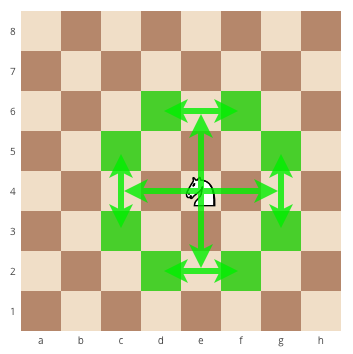
\includegraphics[scale = 0.6]{knight_move.png}
        }
        \caption{Posibles movimientos para el caballo.}
        \label{fig:knight_move}
    \end{figure}



    El problema que queremos resolver es, dada una posici'on inicial y el tama'no del tablero,
    encontrar el camino m'as largo posible utilizando los movimientos del caballo
    y visitando cada casilla a lo m'as una vez.


    \subsection{Artifitial Bee Colony.}\label{section:bee_colony}
    Los algoritmos gen'eticos est'an inspirados en el comportamiento de
    agentes biol'ogicos.

    El algoritmo Bee Colony fue propiesto en el a'no por el investigador InvestigadorName,
    y el funcionamiento intuitivo es el siguiente.

    \textbf{Componentes.}
    \begin{itemize}
        \setlength\itemsep{0em}
        \item Abejas, que se dividen en tres tipos: empleadas, observadoras y exploradoras.
        \item Se tiene un mismo n'umero de abejas de cada tipo.
        \item Fuentes de comida, que representa una posible soluci'on a el problema.
        \item Cada abeja empleada es encargada de una fuente de comida (es decir, tenemos el mismo n'umero de fuentes
                de comida que de abejas empleadas).
        \item Hay una funci'on fitness, que eval'ua la calidad de una fuente de comida.
    \end{itemize}

    \textbf{Metodolog'ia.}
    \begin{itemize}
        \item Se generan fuentes de comida de manera aleatoria.
        \item Se repite un n'umero definido de veces los siguientes pasos
            \begin{itemize}
                \setlength\itemsep{0em}
                \item Todas las abejas empleadas buscan una abeja compa'ra para compartir informaci'on y actualizar
                    la fuente de comida.
                \item Las abejas observadoras toman las fuentes de comida de las abejas empleadas, y seleccionan
                    solo a algunas para actualizar su informaci'on.
                \item Las abejas exploradoras toman las fuentes de comida y las inspeccionan. Si encuentran
                alguna fuente de comida que no puede optimizarse m'as y que se encuentra por debajo de un l'imite
                se descarta y se cambia por una nueva posici'on generada aleatoriamente.

            \end{itemize}

    \end{itemize}

    De manera resumida, las abejas empleadas actualizan todas las fuentes de comida, las observadoras
    actualizan solo algunas soluciones (las m'as optimas al momento) y las exploradoras descartan soluciones
    sub'optimas. Este proceso se repite un n'umero finito de veces y al final observamos
    la soluci'on global.

    \subsection{El papel de la Programaci'on Declarativa.}
    Para las implementaciones de este proyecto se opt'o por el uso de Prolog, lenguaje que pertenece
    al paradigma de la Programaci'on L'ogica. \\
    En Prolog la informaci'on es manejada con hechos y reglas de producci'on.

    Como observaremos en la secci'on ~\ref{section: desarrollo}, una considerable cantidad de operaciones
    que se requieren para los algoritmos consisten en
    \begin{itemize}
        \item Verificar que se cumplan condiciones (por ejemplo, para mutar informaci'on).
        \item Explorar varias posibilidades en un mismo punto (por ejemplo, explorar los posibles movimientos).
    \end{itemize}

    Ambas caracter'isticas est'an intimamente ligadas a la filosof'ia de Prolog, que nos regala la exploraci'on a trav'es
    de su 'arbol de resoluci'on y adem'as tiene el bactracking ya implementado. De igual manera, el enfoque
    procedimental de Prolog consiste en encontrar sustituciones para hacer verdaderos a los predicados.




    \section{Desarrollo.}\label{section: desarrollo}

    \subsection{Representaci'on de la informaci'on.}
    Para todos los m'etodos propuestos a continuaci'on es importante
    entender c'omo estamos representando los distintos
    elementos.

    \begin{itemize}
        \item La posici'on en el tablero es un par  $\mathbf{(X,Y)}$ , donde
        $X$ es el n'umero de la columna y $Y$ el n'umero del rengl'on.
        Ambos valores est'an en un ranto entre $1$ y $N$ (longitud
        del lado del tablero). \\
        Por ejemplo, para un tablero de $3\times 3$ los
        pares para cada posici'on son los siguientes

        \begin{figure}[H]
            \centering
            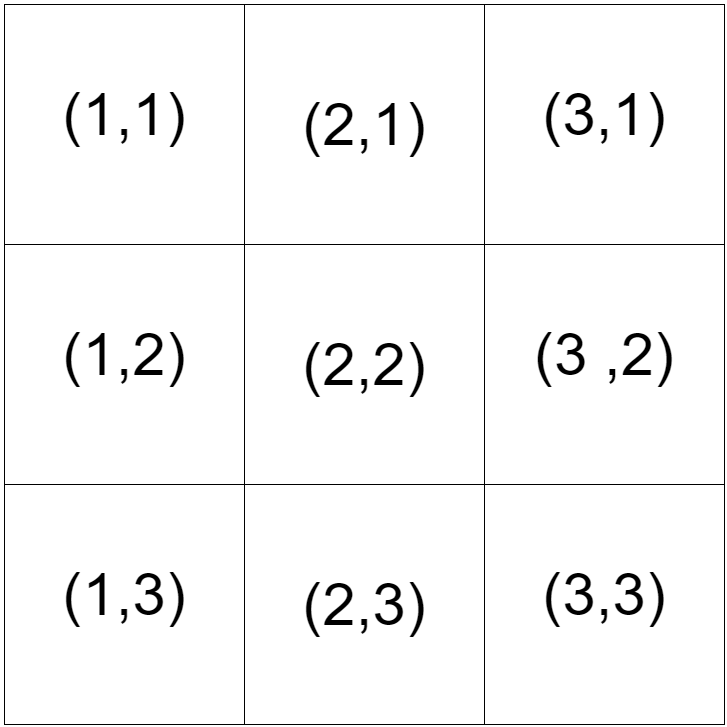
\includegraphics[scale=0.25]{tablero_posiciones.png}
            \caption{Representaci'on de las posiciones en un tablero de $3\times 3$}
            \label{fig: posiciones}
        \end{figure}



        \item Un recorrido se representa con una lista, donde cada elemento
        es una posici'on del tablero. El orden en que se visitan las
        posiciones se lee de izquierda a derecha en la lista.\\
        Por ejemplo, dado el recorrido

        \begin{figure}[H]
            \centering
            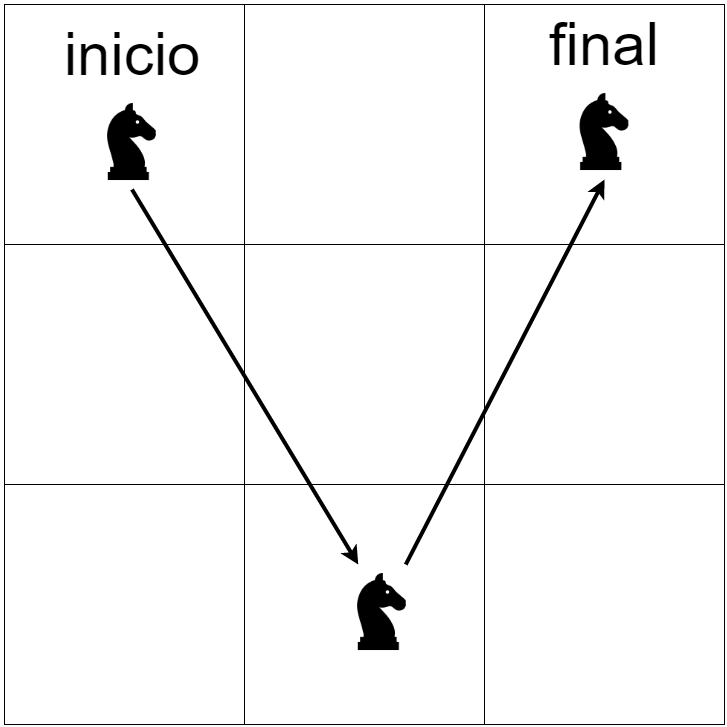
\includegraphics[scale=0.25]{recorrido1.png}
            \caption{Ejemplo de secuencia de movimientos.}
            \label{fig:recorrido1}
        \end{figure}


        su representaci'on es: $[ (1,1) \; ,\; (2,3),\; (3,1) ]$

    \end{itemize}

    Algunos aspectos particulares de cada m'etodo ser'an nombrados
    en su correspondiente secci'on.


    \subsection{Tratando de resolver el problema con fuerza
    bruta.}

    La primera soluci'on propuesta es utilizando una b'usqueda DFS y backtracking.
    La exploraci'on es exhaustiva, con DFS se est'an recorriendo todos los caminos posibles, el backtracking
    es el encargado de volver a puntos anteriores.

    El 'arbol de posibles movimientos y el backtracking es manejado
    gracias a Prolog, pues el recorrido DFS corresponde
    a la exploraci'on que hace Prolog en el 'arbol de resoluci'on.



    Con prolog hacemos una b'usqueda DFS, y al final tomamos
    el recorrido con la mayor longitud.

    Explorar todos los caminos es inviable, para reducir el espacio
    de b'usqueda (y entonces obtener resultados en un tiempo razonable)
    se pueden utilizar muchos m'etodos, uno relativamente
    simple es el descrito en la secci'on siguiente.



    \subsection{Soluci'on con la regla de Warnsfort.}
    La regla de Warnsfort es una heur'istica
    muy famosa propuesta por Warnsfort en .


    \subsection{Adaptando Artifitial Bee Colony para resolver el problema.}

    \subsubsection{Representaci'on de las fuentes de comida.}

    El algoritmo ABC est'a planteado originalmente para problemas con valores continuos. Como nuestro problema es discreto
    se deben realizan unas adaptaciones.


    Los 8 patrones de movimiento del caballo se identificar'an con un n'umero:
    \begin{figure}[H]
        \centering
        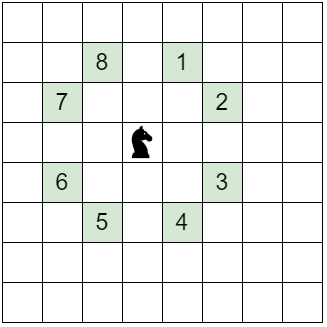
\includegraphics[scale=0.5]{id_move.png}
        \caption{Identificadores de los patrones.}
        \label{fig:id_move}
    \end{figure}



    Las posibles  soluciones para un tablero de $N \times N$
    se representan con una lista de longitud $N^{2} -1 $, donde
    cada elemento de la lista es un n'umero entre $1$ y $8$.

    \begin{figure}[H]
        \centering
        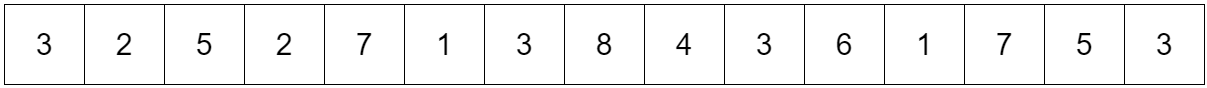
\includegraphics[scale=0.3]{food_source1.png}
        \caption{Ejemplo de posible soluci'on para un tablero de $4\times 4$.}
        \label{fig:food_source1}
    \end{figure}

    El significado operacional de esta secuencia es, dada la posici'on inicial, aplicar el patr'on de movimento
    que se encuentra en la cabeza de la lista, una v'ez llegada a la posici'on destino aplicar el
    patr'on de movimiento que guarda el siguiente elemento de la lsita. \\
    Es claro que las listas pueden guardar movimientos inv'alidos, es decir, al aplicar
    el patr'on de movimiento se regresa a una casilla previamente visitada o se sale del tablero. \\
    El objetivo del algoritmo es entonces maximizar los movimientos v'alidos.


    \subsubsection{Funci'on fitness.}

    La definici'on de nuestra funci'on fitness est'a dada recursivamente:

    \begin{equation} \label{eq: fitness}
        \begin{split}
            f(\; [\;] \;) &= 0 \\
            f( x:xs ) &= \begin{cases}
                            1 + f(xs) &\text{si $x$ es un movimiento v'alido}\\
                            0 &\text{si $x$ es un movimiento inv'alido }
            \end{cases}
        \end{split}
    \end{equation}

    Observe que con esta definici'on entre m'as grande es el valor de la funci'on fitness m'as
    largo es el recorrido que representa la lista.

    \subsubsection{Actualizaci'on de las soluciones.}\label{section: merge}

    Para actualizar la posici'on de una fuente de comida $V_{1}$, primero se
    escoge aleatoriamente una fuente de comida distinta $V_{2}$ , el intercambio
    de informaci'on se realiza obteniendo cuatro fragmentos como se ilustra en
    la siguiente imagen

    \begin{figure}[H]
        \centering
        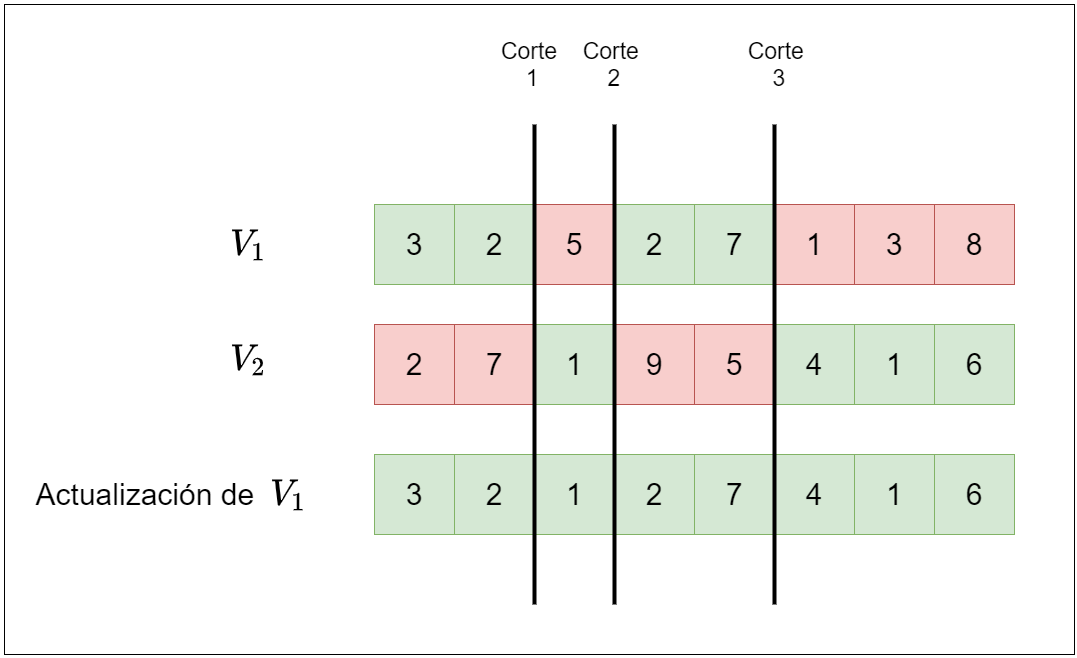
\includegraphics[scale=0.35]{merge.png}
        \caption{Proceso de actualizaci'on de una fuente de comida.}
        \label{fig:merge}
    \end{figure}


    Los puntos de corte son escogidos aleatoriamente.\\
    Recuerde que en todo momento se mantiene una estrategia greedy, cuando la posici'on de una fuente de comida muta se comprueba
    si el valor de la funci'on fitness se incrementa o no, en caso de que no se incremente se descartan los cambios.


    \subsubsection{Algoritmo.}
    Como mencionamos en la secci'on ~\ref{section:bee_colony}, los trabajos realizados por los tres tipos de abejas
    conforman un ciclo de ejecuci'on.

    \textbf{Abejas empeladas.}\\
    Todas las abejas tienen asociada una fuente de comida, de manera aleatoria escogen a una compa'nera y
    actualizan la posici'on de su fuente de comida siguiendo el m'etodo descrito en la subsecci'on ~\ref{section: merge}.

    \textbf{Abejas observadoras.}\\
    Las abejas observadoras toman todas las fuentes de comida que tienen las empleadas, cada fuente
    de comida tendr'a asociada una probabiliad para ser seleccionada.

    La probabilidad de que una fuente de comida $V_i$ sea seleccionada est'a dada por la
    siguiente funci'on
    \begin{equation}\label{eq: selection_function}
        g( V_i ) =  \dfrac{ f(V_i ) } { \displaystyle \sum_{ V_j \in S } f(V_j) }
    \end{equation}

    Donde $S$ es el conjunto de todas las fuentes de comida y $f$ es la funci'on fitness.

    \textbf{Abejas exploradoras.}\\
    Las abejas exploradoras toman todas las fuentes de comida (despu'es de que las observadoras hayan realizado
    sus modificaciones), observan cu'al es el valor m'as grande que toma la funci'on fitness en ese momento para alguna fuente
    de comida,
    llamemos $fit_{max}$ este valor, y para todas las fuentes de comida cuyo
    valor fitness asociado sea menor a $fit_{max}$ se trata de extender la soluci'on.\\
    Observe que el valor fitness nos indica la cantidad de movimientos v'alidos, por lo que
    para una fuente de comida $V_i$, el elemento en la posici'on $f(V_i) + 1$
    es el primer movimiento no v'alido de la secuencia. Las abejas exploradoras tratan de modificar
    este movimiento por otro que sea v'alido, si no existe ning'un movimiento posible v'alido
    entonces $V_i$ es una soluci'on sub'optima (est'a por debajo del l'imite actual y no hay manera
    de que se incremente), por lo que es descartada y reemplazada por una nueva
    fuente de comida generada aleatoriamente. En caso de que s'i exista un movimiento v'alido se realiza la
    modificaci'on a $V_i$ cambiando 'unicamente ese valor. \\

    Adicionalmente a esto, la fuente de comida con mayor fitness value tambi'en se trata de extender (buscando el primer
    movimiento inv'alido y sustituyendolo), sin embargo, en caso de no poder extenderse m'as no se descarta, pues
    es potencialmente la soluci'on global.


    El flujo de ejecuci'on se puede observar como




    \section{Resultados.}
    Las siguientes gr'aficas representan los resultados de ejecutar 50 repeticiones en posiciones distintas
    para tableros de longitud $8 \times 8$.

    \section{Conclusiones.}
    Como podemos observar en el an'alisis de resultados la fuerza bruta
    resulta poco eficiente debido a la complejidad computacional del problema,
    para valores muy peque'nos de n (longitud del lado del tablero)
    el tiempo y poder de c'omputo requerido es inviable. \\
    De los  dos m'etodos que se presentaron como alternativa
    fue la implementaci'on de Artifitial Bee Colony la que dio mejores resultados,
    encontrando caminos m'as largos que la heur'istica de Warnsdorff. \\


    \section{Trabajo futuro.}
    Aunque los resultados obtenidos con el algoritmo ABC son satisfactorios
    hay muchos casos para los que no se encuentra realmente el recorrido m'as largo posible.
    Para mejorar los resultados se deben realizar modificaciones en alguno de los siguientes puntos
    \begin{itemize}
        \item Modificar el n'umero de agentes y el n'umero de iteraciones. De manera m'as general
            encontrar las cotas apropiadas para estos
            valores dependiendo del valor de la variable n.
        \item Modificar la manera en que se comparte la informaci'on entre los agentes.
    \end{itemize}

    Ambos puntos requieren un an'alisis profundo, deben ser implementados y probados
    para saber si mejoran las soluciones.
    Realizar variantes queda fuera del alcance de este proyecto pero
    deben ser tomadas en cuenta para trabajos futuros.


    \section{Disponibilidad de la implementaci'on.}

    Todas las implementaciones presentadas fueron realizadas en Prolog.

    \subsection{C'omo probar la implementaci'on.}

    Los archivos relacionados al proyecto se encuentran disponibles
    en el repositorio\\
    \textbf{
    https://github.com/ciencias-unam/proyecto-final-VladimirSierra
    }

    Le invitamos a leer el archivo README.md para
    c'onocer las instrucciones precisas de ejecuci'on.


    %- Bibliografia
    \printbibliography

\end{document}